%__________________________________________________________________________________________ %
%-------------------------------------------PFC---------------------------------------------%
%__________________________________________________________________________________________ %


%%%%%%%%%%%%%%%%%%%%%%%%%%%%%%  PREAMBULO  %%%%%%%%%%%%%%%%%%%%%%%%%%%%%%%%%%%%%
% ----------------------Especificaciones de dise�o---------------------------- %

\NeedsTeXFormat{LaTeX2e}
\documentclass[12pt]{book}

\usepackage{a4}
\usepackage[Lenny]{fncychap}    % Estilos para capitulos
\usepackage{fancyhdr}           % Estilos para cabeceras
%\usepackage[spanish]{babel}
%usepackage[latin1]{inputenc}

% Para no tener problemas con las tildes
\usepackage[utf8]{inputenc}
\usepackage[english]{babel}

\usepackage{epsfig}
\usepackage{subfig}
\usepackage{epstopdf}
\usepackage{caption}
\usepackage{keyval}
\usepackage{graphicx}
\usepackage{float}              % Para poner las imags en cualquier sitio
\usepackage{listings}
\usepackage{color}
\usepackage{textcomp}
\usepackage{verbatim}
\usepackage{exceltex}



\definecolor{listinggray}{gray}{0.98}
\definecolor{lbcolor}{rgb}{0.98,0.98,0.98}
\lstset{
	backgroundcolor=\color{lbcolor},
	tabsize=3,
	rulecolor=,
	language=matlab,
	basicstyle=\footnotesize\sffamily,
	aboveskip={1.5\baselineskip},
	belowskip={1.5\baselineskip},
	columns=fixed,
	showstringspaces=false,
	extendedchars=true,
	breaklines=true,
	prebreak = \raisebox{5ex}[5ex][5ex]{\ensuremath{\hookleftarrow}},
	frame=none,
	showtabs=false,
	showspaces=false,
	showstringspaces=false,
	identifierstyle=\ttfamily,
	keywordstyle=\color[rgb]{0,0,1},
	commentstyle=\color[rgb]{0.133,0.545,0.133},
	stringstyle=\color[rgb]{0.627,0.126,0.941},
}

\usepackage[numbers,sort&compress,comma]{natbib}	% Modo de poner la bibliograf�a
\usepackage{verbatim}      %  \begin{comment}...\end{comment}
\usepackage{subeqnarray}   % equationarray with numbers 1a, 1b, ...
\usepackage{bbm}           % Para s�mbolo tipo n�meros reales. Ej: \bbm{R}
\usepackage{longtable}     % Para tablas largas de m�s de una p�gina
\usepackage{rotating}
\usepackage{psfrag}        % Para cambiar fragmentos de text en .eps por otro en latex
\usepackage{pifont}        % Para otros s�mbolos
\usepackage{fancybox}      % Para encuadrar texto en recuadros
\usepackage{amsmath}       % Mejora la calidad de las formulas
\usepackage{amsfonts}
\usepackage [linktocpage]{hyperref}      % Para enlaces de hipertexto
\usepackage{amssymb,amsfonts}
\usepackage{multirow}
\usepackage{booktabs}
\usepackage{color}
\usepackage{longtable}
\usepackage{float}
\usepackage{array}




\setcounter{tocdepth}{2}             % toc = table of contents. Para definir niveles del �ndice
\setcounter{secnumdepth}{5}          % Hasta cu�ndo se enumeran los caps, seccs, etc


\setlength{\topmargin}{-1.1cm}        % margen por arriba
\setlength{\parskip}{\baselineskip}
\setlength{\parskip}{0.3cm}          % Espacio entre parrafos
\setlength{\textwidth}{16.5cm}       % Ancho del �rea imprimible	
\setlength{\evensidemargin}{-0.4cm}  % Margen izdo en p�ginas pares
\setlength{\oddsidemargin}{0.3cm}    % Margen izdo en p�ginas impares
% evensidemargin = -oddsidemargin !!!

\setlength{\headsep}{1.0cm}
\setlength{\headheight}{3ex}
\setlength{\footnotesep}{5mm}
%\setlength{\mathindent}{1.0cm}       % Controla el espacio entre margen y ec si no est� centrada


%%% Definitionen f�r Fancy Headings
%\renewcommand{\baselinestretch}{3mm}
%\renewcommand{\labelenumi}{\roman{enumi}.}
%\renewcommand{\chaptermark}[1]{\markboth{#1}{}}
%\renewcommand{\sectionmark}[1]{\markright{\thesection\ #1}{}}
\renewcommand{\labelitemi}{$\bullet$}
\renewcommand{\labelitemii}{$\diamond$}
\renewcommand{\labelitemiii}{$\cdot$}

\lhead[\fancyplain{}{\thepage}]{\fancyplain{}{\sl\nouppercase\rightmark}}
\rhead[\fancyplain{}{\sl\nouppercase\leftmark}]{\fancyplain{}{\thepage}}
\cfoot{}
\pagestyle{fancyplain}  		% normale Kopfzeile; ohne Seitenzahl: empty

% Formato de capitulos
\ChTitleVar{\sf\Huge} % Tama�o de la letra del nombre del cap
\ChTitleAsIs


%%% Comando para quitar encabezado y pie de las pag en blanco
\newcommand{\clearemptydoublepage}
{\newpage{\pagestyle{empty}\cleardoublepage}}

\newcommand{\R}{\mathbb{R}}
\newcommand{\x}{\mathbf{x}}
\newcommand{\grad}{\hspace{-2mm}$\phantom{a}^{\circ}$} %para los grados centigrados

%%% Abstract
\newenvironment{abstract}
{\begin{center}
		\begin{minipage}{0.8\textwidth}
			\slshape}
		{\end{minipage}
	\end{center}}
	
	
	\typeout{ }
	\typeout{----------------------------------------------------------------------}
	\typeout{ }
	
	



%%%%%%%%%%%%%%%%%%%%%%%%%%%%%%  DOCUMENTO  %%%%%%%%%%%%%%%%%%%%%%%%%%%%%%%%%%%%%
%-------------------------Cuerpo del documento---------------------------------%


\begin{document}
	\renewcommand{\contentsname}{Contents}
	\renewcommand{\listfigurename}{List of figures}
	\renewcommand{\listtablename}{List of tables}
	\pagenumbering{roman}    % Numeraci�n de p�ginas con num romanos
	\setcounter{page}{1}      % Establece la siguiente p�gina como la 1
	\begin{titlepage}
\label{ch:cover}
\begin{center}


\vspace{2cm}

%\begin{figure}[h]
%	\centering
%	
\epsfig{file=figures/ugr.eps, width=7cm}
%	\label{fig:ugr2}
%\end{figure}


\vspace{1cm}
\textbf{\Huge{GaitWatch: User Manual}}
\vspace{1.2cm}
\begin{figure}[H]
\centering
\includegraphics[width=0.5\textwidth]{figures/GW_cover.jpg}
\end{figure}

\end{center}

\vspace{0.5cm}
 

\begin{center}Prof. Dr. med. Kai B\"otzel$^{a}$\\ 
Dr. Alberto Olivares Vicente$^{b}$\\\vspace{0.6cm}
$^{a}$ \textit{Department of Neurology, Ludwig-Maximilians University, Munich, Germany.}\\
$^{b}$ \textit{Department of Signal Theory, Telematics and Communications, University of Granada, Granada, Spain.}\\
\end{center}

\vspace{1cm}
\begin{figure}[H]
\raggedleft
\includegraphics[width=0.3\textwidth]{figures/lmu_logo.png}
\includegraphics[width=0.3\textwidth]{figures/ugr_logo.jpg}
\end{figure}

\end{titlepage}
		% Inclu�mos la portada en espa�ol
	\clearemptydoublepage
	
	%Declaración
%--------

\begin{titlepage}
\label{ch:Statement}
\vspace{2cm}

\noindent  D. Alberto Olivares Vicente, profesor  del dpto. de Teoría de la Señal, Telemática y Comunicaciones, como director del Proyecto Fin de Carrera de Dª. Verónica Torres Sánchez,

\vspace{2cm}
\noindent Informan:

\vspace{1.5cm}
\noindent Que el presente trabajo, titulado:

\noindent \textbf{Comparison of Posturographic Body-sway Measurements with Inertial Data of Parkinson Patients.}

\noindent Ha sido realizado y redactado por el mencionado alumno bajo nuestra dirección, y con esta fecha autorizamos a su presentación.
\vspace{3.5cm}

\noindent Granada, a XX de XXX de 2015 Fdo:

\vspace{6.5cm}
\noindent D. Alberto Olivares Vicente  

\end{titlepage}       % Incluimos la declaración del proyecto
	\clearemptydoublepage
	\begin{titlepage}
\label{ch:acknowledgements}
{ \huge \bfseries Acknowledgements \\[0.4cm] }


First and foremost, I would like to thank Dr Alberto Olivares Vicente and Juan Manuel Górriz Sáez for supervising this work, his assistance and most especially for his continuous motivation and encouragement. 

My appreciation as well to Dr. Kai Bötzel and his team from the Department of Neurology of the Klinikum Grosshadern of Munich for suggesting the project, his counseling and for providing the necessary database.

Thanks to Robin Weiss for his suggestions, his great ideas and knowledge, his jokes when the work was being  hard and, in short, for helping me along this Project.

Special thanks go to my friends for valuing my work, encouraging me every day, their advices and making me smile with their crazy things. Of course, many thanks go to my friend and flatmate, for putting up with me in the work nights and making me laugh with their positive music.

Finally, I am deeply grateful to my family, for giving me the opportunity to study, respecting all my decisions and their motivation and affection.


\end{titlepage}       % Incluimos agradecimientos
	\clearemptydoublepage
	\begin{titlepage}
\label{ch:abstract}
{ \huge \bfseries Abstract \\[0.4cm] }

Posturographic Body-Sway Measurements are increasingly important in many fields of modern medicine, sport activities and teleassistance.  Postural instability is an important contributor to incapacitation in elderly people and patients with neurological or motion disorders like people with Parkinson’s disease.

This work describes the development  of a comparative study between several systems to measure the Posturographic Body-sway and techniques and procedures to extract features of them. Along this document we describe, firstly, the most common  instrumentation in these kind of experiments as well as the methods  used for data analysis of Anticipatory Postural Adjustment (APA) in Parkison patients. Secondly, we will introduce a general description of all devices used to data gathering  for the development of  this project. These devices are: Gait Watch, a system based in inertial sensors for gait monitoring, Force Platform , a system for force measurements and Qualisys System, a system that uses speed digital cameras and marker attached.

The core of the project consists of comparating the signals obtained from the systems mentioned above. In the first place, we are going to compare the GW anf FP signals to determine whether we can obtain the same information of both systems and we can use the inertial sensors in place of platforms of force. To do this, we will carry out the synchronisation of the signals, analysis of APA and the feature extraction of these signals. In this last aspect, we focus in PCA algorithm because it allows us the reduction of redundant information and the interpretation of multiple gait signals. In second place, we are going to analyse the Gait Watch system in comparison with the Qualisys Optical motion tracker. In this case, we will calculate the pitch angle for both systems. We will compare features like ‘stride time’ and angle. Before doing this, we explain  the configuration of Qualisys System and how we figure out the angle for each point of time. In addition, we will do a feature extraction using both PCA and PLS algorithms and classification of data force in another different experiment with Parkinson patient and healthy people. This allows us to determine the accuracy of force data for the diagnostic of this disease.

Finally, we present a summary of the different fields of applications related with heathcare and a brief  business plan where we explain a discription of a business idea and the most important aspect to take into account.

\end{titlepage}       % Incluimos resumen
	\clearemptydoublepage
	
\begin{titlepage}
\label{ch:abbrevations}
{ \huge \bfseries Abbrevations \\[0.4cm] }


\end{titlepage}       % Incluimos abreviaciones
	\clearemptydoublepage
	
	\tableofcontents          % Pone índice
   \listoffigures		   	% Crea la lista de figuras
   \listoftables			% Crea la lista de tablas
	\clearemptydoublepage

	

	\clearemptydoublepage
	\chapter{Introduction}
\label{ch:Introduction}

Monitoring and assessment of human body motion, in particular the analysis of gait, has become an integral part of medical diagnosis, therapy techniques, and rehabilitation \cite{tao_gait_2012}. \emph{Gait analysis} involves the measurement and assessment of quantitative parameters that characterise human locomotion. First research in this field was conducted in the late 19\textsuperscript{th} century \cite{tao_gait_2012}. The quantitative data enable physicians to diagnose a variety of medical conditions, validate treatment success, set goals in rehabilitation and regularly alter them when necessary. However, standard gait analysis based on multi-camera motion capture systems and force platforms require specialised gait laboratories, expensive equipment, and lengthy setup times. Moreover, the assessments of gait based on measurements performed in clinical settings might not be truly representative \cite{bonato_advances_2005}.

Unobtrusive wearable sensors mitigate the aforementioned limitations. Low cost sensors have been employed in clinical and home environments to constantly monitor the movements of patients \cite{godfrey_direct_2008}. The progressive miniaturisation of inertial and magnetic field sensors has made them more acceptable to patients and has consequently lead to an increasingly pervasive adoption for medical applications \cite{wee_soon_ambulatory_2008}, especially in the truly representative home environment.  Among others, wearable inertial and magnetic sensors are used to assess \emph{gait kinematics}. An extensive description is presented in Section \ref{sec:MARG_sensors_medical}. \emph{Kinematics} is a branch of classical mechanics, which is concerned with motion of objects without reference to the forces causing the motion. Position, velocity and acceleration are of particular interest in kinematics.

Determining the position of the legs is essential in gait analysis. The position, i.\,e. the orientation, can be estimated from inertial data. For the application in health care accurate orientation estimates are crucial. A high degree of precision based on data from miniaturised sensors necessitates adequate signal processing, in order to mitigate the influence of disruptive factors, such as bias instability and noise, among others. The signal processing of inertial and magnetic data encompasses calibration, adaptive filtering, and sensor fusion. The latter two are a part of this work.

\section{Motivation}

Gait analysis provides a powerful means to derive diagnostic information about the functioning of the musculoskeletal, vestibular, and central and peripheral nervous system \cite{bennett_extended_2013}. Accurate orientation estimation of the extremities by means of wearable inertial and magnetic field sensors allows objective assessment of human gait and can therefore benefit medical applications without the aforementioned constraints of camera based motion capture systems. A more reliable and more precise orientation estimation would enable an even more informative gait analysis. A multitude of applications in the medical field would profit from such an enhanced gait analysis \cite{wong_clinical_2007}. The direct relation to health care and the resulting possibility to improve the quality of life of many patients was the motivation for this thesis.

\section{Goals}

The goal of this thesis was implementing a new Kalman filter based orientation algorithm proposed by \citeauthor{bennett_motion_2014} in \cite{bennett_motion_2014}. Thus the estimation of orientation angles of the human leg by means of inertial and magnetic sensors should be improved. The filter algorithm should be implemented using \textsc{Matlab}\textsuperscript{\textregistered} and validated against existing algorithms by comparing their respective \gls{RMSE}. An existing system for human body motion analysis based on wearable sensors was available, so that no new hardware had to be developed to gather the movement data. A detailed description of the so-called GaitWatch system is found at the end of Chapter \ref{ch:MARG}.

\section{Methodology}

This document presents my work within the overall project in a chronological order. Subsequent to the previous introductory overview of the topic and the definition of the project objectives, this chapter ends with a description of the state of the art. To accomplish the tasks defined in the previous section, I had to acquire knowledge regarding various subjects. Chapters 2 to 4 outline the necessary fundamentals of MARG sensors, orientation estimation and digital filters, respectively.  This enables comprehension of the overall project, even for readers that are not familiar with some of the subjects. Those readers are referred to Chapters 2 to 4 at this point, before reading the state of the art. The actual implementation of the Kalman filter, including a prior theoretical design is given in Chapter 5. This chapter also encompasses the experimental setup, the results and a discussion of the latter. Finally, Chapter 6 covers conclusions and future work.

I implemented the filter algorithm in the numerical computing environment \textsc{Matlab}\textsuperscript{\textregistered}. As additional means to communicate with my supervisor and in order to enable him to follow the progress of my work at any time we used Pivotal Tracker, a tool for agile project management, and GitHub, a repository hosting service based on the distributed version control system Git. This thesis was written in \LaTeX{}.
 
\section{State of the Art}\label{sec:state_of_the_art}

There are several research works in the literature dealing with orientation estimation by means of inertial sensors. Kalman filters have been used successfully to improve the estimation of orientation angles from inertial data. The state of the art at the commencement of the project is described below. Subsequently, applications of wearable inertial sensors in health care and current attempts to revolutionise medical research assisted by those sensors are presented.

\subsection{Kalman Filtering in Orientation Estimation} \label{sec:state_of_the_art_kalman}

Considering the fact that inertial and magnetic field sensors are used to establish objective body motion parameters that affect medical diagnosis, therapy, and rehabilitation, the necessity of a high level of accuracy becomes obvious. In order to obtain precise orientation estimates from sensor data it is essential to mitigate the effects of measurement noise and to combine the advantages of different  sensors through sensor fusion. Therefore, a wide variety of Kalman filter algorithms have been developed in the literature. It is common practice to fuse accelerometer and gyroscope measurements to mitigate their respective drawbacks and thus obtain more accurate orientation estimates.

\citeauthor{Luinge_orientation_acc_gyro_99} \cite{Luinge_orientation_acc_gyro_99} alleged that the gravitational component of the acceleration signal has a greater magnitude than the component caused by motion for many human movements. They estimated the tilt angle, which is defined as the angle between the sensor axes and the vertical. The separate estimates from an accelerometer and a gyroscopes were fused with a Kalman filter. To test their method they moved the sensors around by hand for 30 seconds and then put it in a known position. They orientation obtained by integrating the angular rate only served as a reference. They concluded that a fusion of accelerometer and gyroscope signals accounts for a considerable improvement of the orientation estimation. This approach lacks of dynamical comparison since it only compares the errors at specific static positions.

Due to human motion intensity usually being subject to change, \citeauthor{olivares_vicente_signal_2013} implemented a \emph{gated Kalman filter} in \cite{olivares_vicente_signal_2013}. They modelled linear acceleration during intense motion as noise and improved the performance of the Kalman filter by dynamically adjusting the variance of both the process and measurement noise, according to the motion intensity. Therefore, they applied a \gls{LTSD} and set the variance between two predefined values. Then, the gated Kalman filter fused information from the accelerometer and the gyroscope signals. With this method they improved the adapting capability of the filter and consequently the precision of the orientation estimation.

\citeauthor{bennett_motion_2014} demonstrated in \cite{bennett_motion_2014} that accelerometer angle estimates are inaccurate for typical motions of the leg. They affirmed the need to decouple the acceleration due to motion from the acceleration due to gravity, since the former cannot be neglected during fast motions. Therefore, they deployed a \emph{kinematic model} of the leg to determine the acceleration that occurs due to motion and corrected the acceleration signal accordingly. An extended Kalman filter fused the corrected acceleration data with measurements of a gyroscope. This method improved upon the raw acceleration method during motion and at rest by an 83\% smaller \gls{RMSE}. Their proposed approach is the foundation of the filter algorithm implemented in Section \ref{sec:theoretical_design}.

\subsection{Wearable Sensors in Health Care}\label{sec:MARG_sensors_medical}

Inertial sensors can be found in smart phones, fitness trackers, and other wearable devices, among others. With increasing capability of body sensor networks and wearable computing, they have become prevalent in research environments for estimation and tracking of human body motion \cite{bennett_motion_2014}. They are used in activity monitoring \cite{veltink_detection_96, najafi_ambulatory_03, ermes_sports_08}, rehabilitation \cite{giggins_rehabilitation_13, lupinski_ligament_11}, sports training \cite{bonnet_squat_13, ermes_sports_08}, and localisation \cite{hoflinger_localization_13, Bennett_distance_13}.

Many neurodegenerative diseases such as, for instance, Parkinson's disease, impair stable stance and gait and reduce the patient's mobility. Thus, they diminish the quality of life significantly. \emph{Parkinson's disease} is a movement disorder that is characterised by marked slow movements, tremors, and unstable posture. Especially in advanced stages of the disease many patients exhibit an episodic, brief inability to step, which delays gait initiation or interrupts ongoing gait. This phenomenon is called freezing of gait. With the progression of the disease, Parkinson's patients are increasingly dependent on help from others to accomplish daily tasks. One of the most reliable diagnostic criterion of the disease is gait \cite{tao_gait_2012}. Hence, wearable motion sensors have been used successfully to classify the severity of the disease objectively \cite{mancini_anticipatory_2009, palmerini_feature_2011, klerk_long-term_2009}.

Stroke patients, who regained their walking ability, need to undergo rehabilitation to recover their independent mobility. Ambulatory gait analysis provides a means to assess the function of the lower extremities of hemiparetic post-stroke patients and follow the progress of rehabilitation \cite{tao_gait_2012, saremi_reliability_2006}. In addition, the presence of neurologic gait abnormalities is used as a significant predictor of the risk of development of dementia \cite{verghese_dementia_2002}. Also, emergency falls of elderly people can be detected \cite{bourke_threshold-based_2008, bourke_assessment-waist_2010, bourke_fall_detection_2008}.

\subsection{The Impact of Wearable Sensors on Medical Research}

The fact that most of the current smartphones come equipped with inertial and magnetic sensors and powerful processor has opened up new possibilities for medical research. The number of smartphones across the globe is predicted to surpass two billion in 2016 \cite{emarketer_smartphones}. Recently, large companies have developed software that takes advantage of the associated potential to revolutionise medical research.

In August 2014, the Michael J. Fox Foundation for Parkinson’s Research and Intel Corporation \cite{Intel_2013} announced a collaborative research study on objective measurement of Parkinson symptoms. They aim to collect movement data of thousands of patients twenty-four seven at over 300 samples per second by means of unobtrusive wearable devices and store them on a big data analytics platform. The data platform, deployed on a cloud infrastructure, supports an analytics application that processes the data and detects changes in real time. Thus, by detecting anomalies, the progression of the disease can be measured objectively without the need for scientists to focus on the underlying computing technologies. Physicians and researchers are intended to have access to the data as well as be able to submit their own anonymised patient data for analysis. According to \cite{Intel_2013} the correlation of data that quantifies symptoms such as slowness of movement, tremor, and sleep quality with molecular data could advance drug development and provide a deeper insight into the clinical course of Parkinson's disease.

In March 2015, \citeauthor{Apple_2015} announced a platform-independent, open source software framework called ResearchKit \cite{Apple_2015} that, amongst others, takes advantage of the MARG sensors in the iPhone to track movement of patients in daily life. Thus medical researchers obtain robust data with far more regularity than it was possible when patients complete tasks at hospitals or other research facilities in irregularly intervals. Moreover, according to \citeauthor{Apple_2015} ResearchKit simplifies recruiting participants from all over the world, which results in a more varied study group that provides a more useful representation of the population. Together with the University of Rochester and Sage Bionetworks they announced the iPhone app `mPower' \cite{mpower}, which measures balance and gait of Parkinson patients to help researchers better understand how various symptoms are connected to Parkinson's disease.


	\clearemptydoublepage
	\chapter{Hardware Description}
\label{ch:Hardware}
Along this chapter we will introduce a general description of all devices used to data gathering for the development of this project.


It should be noted at this point that there are two clearly differentiated parts. In the first of them, we work with Force Plate and GaitWatch data, taking out their characteristic signals and synchronising them. In the second of them, we work jointly with Gait Watch and Qualisys System data for the purpose of comparing the accuracy in the calculated orientation angles.


\section{GaitWatch}

GaitWatch is an Inertial Measurement Unit (IMU) designed for gait monitoring of patients. It was developed by Prof. Dr. Med. Kai Bötzel at the Department of Neurology of Ludwig-Maximilians University in Munich in conjunction with Dr. Alberto Olivares Vicente from the Department of Signal Theory, Telematics and Communications of the University of Granada \cite{OlivaresBotzel2013}.

The system is composed of the central processing unit and
a set of measuring units which are wired to it. The measuring units are 
placed in the patients’ thighs, shanks, arms and trunk.

\begin{figure}[H]
	\centering
	\epsfig{file=imagenes/GeneralDiagramGW, width=7cm}
	\caption{General Diagram of the Gait Watch.}
	\label{fig:diagram}
\end{figure}

The central processing unit has a microcontroller is in charge of gathering the data from the external measurement units and writing it to the memory card. So, this central unit is placed in the trunk inside a box and it contains an AL-XAVRB board with an AVRATxmega processor which contains the necessary embedded firmware to gather the data from all the measurement units and store it in a microSD card. Also, the trunk box contains some embedded magnetic and inertial sensors.

\begin{figure}[H]
	\centering
	\epsfig{file=imagenes/devicesGW, width=7cm}
	\caption{Devices used in Gait Watch System.}
	\label{fig:devicesGW}
\end{figure}

There are three different kinds of external units with the following components:
\begin{itemize}
	\item Type A (thighs and shanks): 
	\begin{itemize}
		\item IMU 5 from Sparkfun. IMU 5 contains an IDG500  biaxial gyroscope (from which only Y axis is actually used) with a measurement range of $\pm500deg/s$ and a $\pm3g$ triaxial accelerometer, ADXL335 .
	\end{itemize}
	\item Type B (arms):
	\begin{itemize}
		\item IDG500  biaxial $\pm500deg/s$ gyroscope.
	\end{itemize}
	\item Type C (trunk box):
	\begin{itemize}
		\item ADXL345  triaxial accelerometer with programmable range ($\pm16g/\pm8g/\pm4g/\pm2g$).
		\item IMU3000 triaxial gyroscope with programmable range ($\pm250/\pm500/\pm1000/\pm3000 (deg/s)$).
		\item Micromag3  triaxial magnetometer ($\pm11Gauss$).
	\end{itemize}
\end{itemize}


\section{Force Platform}
Force Plate (FDM-S Multifunction Force-measuring Plate, Zebris) is a System for force measurement and it can be used as a complete measuring unit for stance and roll-off analysis \cite{forceplate}.

This platform consist of a large number of force sensors and enables the distribution of static and dynamic forces under the feet to be analyzed during stance and gait (65x40 cells of sensors). As a result, foot deformities, foot function and posture can be analysed and are available as an evaluation report \cite{forceplate}.

Therefore, this gathered information can be used afterward to analyse the postural adjustments with the right software.

\begin{figure}[H]
	\centering
	\epsfig{file=imagenes/FDMS_Zebris, width=7cm}
	\caption{Platform used to analyse the force under the feet.}
	\label{fig:FDMS}
\end{figure}


\section{Qualisys System}
The Qualisys optical motion tracker is a system that uses high speed digital cameras to capture the motion of a measurement object with passive or active markers attached \cite{OlivaresBotzel2013}.

This technology is used by researchers and clinicians to undertand the basic for human motion or improve treatment during a reabilitation process. Also, it used in industrial applications, for example, the interior design of a car can be improved by using this System to evaluate the confort and safety factors for the car driver \cite{Qualisys}.

The technology is precise and delivers high quality data to the observer in real-time. The core component of Qualisys System is one or more infrared optical cameras that emit a beam of infrared light. Also, there are small retro-reflective markers on a object or person. When the cameras emit infrared light onto the markers, these reflect the light back to the camera sensor and this information is used to calculate the position with high spatial resolution  \cite{Qualisys}. The used system has eight cameras which are distributed around a room.

\begin{figure}[H]
	\centering
	\epsfig{file=imagenes/QualysisSystem, width=7cm}
	\caption{Qualisys optical motion tracker.}
	\label{fig:QS}
\end{figure}

The provided software tools allows to perform basic motion calculations,
such as speed, acceleration, rotation and angle, as well as other more complex
calculations. The precision of this system allows its use as a reference system to evaluate portable motion tracking systems such as the GaitWatch  \cite{OlivaresBotzel2013}.

	\clearemptydoublepage
	\chapter{Gait Watch and Force Plate signals processing}
\label{ch:GWandFP}

\section{Introduction and chapter's structure}
Along this chapter we will introduce the protocol used to obtain the Gait Watch and Force Plate signals as well as the developed software to synchronise and analyse the signals that characterise the anticipatory postural adjustments before gait.

On the one hand, we carry out the synchronisation between the signal from inertial sensors (Gait Watch) and the force signals from the platform. It's very important for comparing both devices, determining the differences and similarities and finally resolving if we can obtain the same information from both systems.

On the other hand, we’ll analise the most interesting signals to characterise the APAs, obtaining the parameters of them which may be of interest.


\section{Data gathering Protocol}
Prior to start of data gathering, it’s necessary to set up the protocol for procedure that patients have to carry out while the data are recorded. The establishing this procedure is very important so that the synchronisation works properly because we have to identify a clear movement in both signals to match one signal with the other at the same time.
In addition, the realised movements must be representatives to obtain conclusive data which help us to extract characteristics for the purpose of identify differences between patients and control subjects subsequently.

The steps followed by the patients are detailed hereafter:

1.	Subject stands in front of the Force Plate.

2.	Gait watch record starts for data gathering.

3.	Force plate record starts for data gathering.

4.	Subject makes a step onto the platform.

5.	Subject stands on the platform a variable time between 2 and 10 seconds.

6.	Subject makes some step  forward and turns left to stand in front of the platform again.

This procedure is repeated ten times by each subject in order to characterise better the movement made.
It’s important to clarify that the GaitWatch recording contains all these ten episodes ( in other cases more) and the platform recording only contains one episode each. So, this is a fact that we have to consider to do the synchronisation.

\section{Synchronisation}

\subsection{Introduction and chapter's structure}
One of the most important aspects whether you have data acquired from multiples devices or channels is the synchronisation. If these data are not appropriately correlated or synchronised, the analysis and conclusions from your use will be erroneous. Also, it’s very important doing all automatically when you have a data on a broad scale.
Therefore, the following sections explain how the information has been obtained and processed automatically, as well as what features have been calculated to characterise the movements of the patients and to carry out the synchronisation between the Force Plate signals and GaitWatch signals. This content is superficially depicted in figure XX.

\begin{figure}[H]
	\centering
	\epsfig{file=imagenes/diagramSynchronisation, width=8cm}
	\caption{Diagram of the Synchronisation's progress.}
	\label{fig:arte1}
\end{figure}

\subsection{Design of developed code  in Matlab}
\subsubsection{Selection, reading and obtaining of information from the excel file}
All patients data , that is, the different files have been generated after the gathering (  of the force plate as well as Gait Watch), gathering date, duration of the experiment and other observations are saved in a Excel file. 

In order to automate all as much as possible, the code is in charge of extraction of the necessary data (files names) to carry out the appropriate calculations for each patient. This is done once the Excel file has been selected, thus, it have to have a specific structure to be able to read the data correctly.

At the end of this fraction of code, we save all file names of both systems (force plate and Gait Watch) corresponding to each patient, in order to access and extract them posteriorly.

\subsubsection{Extraction of the forceplate data}
As we said before, the  force plate data files are recorded independently each others, that is, there is a *.txt file for each repeat.
Each file contains the force data of the toes and heels of both feet. It really realises a distribution of the sensors to cover these four segments. Every measure is obtained for each point of time according to the sample frequency. Also, this file contains the force data from each cell that is part of platform in each frame.

Once we recover this data, some parameters are calculated for the movement characterization carried out over the platform. 

\begin{itemize}
	\item \textbf{Midline}: it represents the midline between both feet. This is important to find the gap between feet and it gives us a idea of their position in the platform. Thus, we carry out the sum of cells force in the anterior-posterior direction. So, this line is in the minimum between two maximum corresponding to the position of both feet. We use this parameter to calculate the center of pressure.
	
	\item \textbf{The total force in the platform for each point of time}: This signal is useful to do the synchronisation due to we can determine clearer when the patient touches the plate.
	
	\item \textbf{Antero-posterior COP}: center of pressure forward-backward direction.
	
	\item \textbf{Medio-lateral  COP}: center of pressure  in right and left direction.
	
	
\end{itemize}

Center of pressure can be expressed as follows:

\begin{equation}
	\label{COP}
	R=\sum_{i}^{n}m_{i}r_{i}
\end{equation}


Where R is the “Center of pressure”, M is the total force and mi are the force that are located in space with coordinated ri, in this case, in the plane. This location (ri) is calculate with respect to the midline.

These signals help us to characterise Anticipatory Postural Adjustments  before gait.  APAs indicate the movement or swinging of body before walk or carry out some movement. Thus, these are the interesting  measures to compare between each repeat as well as each patients to characterise the movement, determine if there is a pattern and figure out the differences and similarities between them.

All these signals are saved for each cycle in a single variable corresponding to the patient.


\subsubsection{Calibration of the GaitWatch data}
When we are working with sensors, calibration is one of the most important aspect that needs to be carried out. Prior to the calibration process,
the information at the sensors  will be a signal composed of integer
numbers  or real numbers bounded into a range which is determined by the precision of the sensors and converters. These numeric values lack of physical value, so it is absolutely necessary to convert them into a scale that can be measured in physical units.

The sensors present several errors due to some effects like scale factor may not be linear or the triad isn’t perfectly orthogonal. To remove these undesired effects, the software include a model to compensate this before the calibration. 
To do so, we have used the code made by Dr. Alberto Olivares Vicente in his doctoral thesis, with minor modifications of his work.

Besides the unwanted effects mentioned above, the output of magnetometers is distorted by wide band measurement noise appearing several large peaks of noise in the signals. To remove this automatically, we used a threshold considering that these peaks are much greater than the mean of the signal.


The erroneus values in the magnetometer signal are removed sustituting these samples by the subsequent value unless the erroneous value is in the last position of the singal, in which case it is substituted by the preceding value.

\subsubsection{Synchronisation}	
\subsection{Results discurssion}


\section{APA analysis}


	\clearemptydoublepage
	\chapter{Gait Watch and Qualisys Optica motion tracker}
\label{ch:GWandQS}

\section{Introduction and chapter's structure}
After explaining and comparing both Gait Watch and Force Plate systems, we proceed now to do an analysis of the differences and similarities between Gait Watch and the Qualisys Optical motion tracker.

It has been demonstrated that Qualisys System is an accurate system to analyse the body movements and it can be used in several applications. However, this system has a lot of constraints like the possibility of application scope.

Thus, we are going to do a comparison with the Gait Watch system, a system based on inertial sensors being more portable and cheaper.
Along this chapter we will explain how the pitch angle has been calculated using the Qualisys System. That is, we will compare with the angles obtained through inertial sensors.


\section{Computing Euler angles using Qualisys System}
To compute the Euler angle, the subject is wearing two infrared markers per segment placed on both thighs and shanks. The infrared optical cameras emit infrared light and this reflects in the markers placed over the body allowing to know the position of the markers.

The pitch angle of such segment is computed between the vector defined by the upper and lower markers and the vector normal to the Earth’s surface. To be able to compute it we first have to define a third point which has the same X coordinate as the lower marker and the same Z coordinate as the upper marker. This will define a right triangle in which one of the contiguous cathetus is normal to the Earth’s surface and the hypotenuse is defined by the line between the upper and the lower point. Therefore, by calculating the arctangent we can easily find the angle of the right triangle, which is, in turn, the pitch angle\cite{OlivaresBotzel2013}. We can see this in \ref{fig:pitchQS}

\begin{figure}[H]
	\centering
	\epsfig{file=imagenes/pitchQS, width=1\textwidth}
	\caption{Diagram of the pitch computation using the Qualisys System \cite{OlivaresBotzel2013}.}
	\label{fig:pitchQS}
\end{figure}

Thus, the pitch angle is computed as follows:

\begin{equation}
\label{angleQS1}
	\theta_{QS}= arctang(\frac{a}{b})
\end{equation}

\begin{equation}
\label{angleQS2}
	a= \sqrt{(x_{upper}-x_{lower})^{2} + (z_{upper}-z_{upper})^{2} }
\end{equation}

\begin{equation}
\label{angleQS3}
	b= \sqrt{(x_{lower}-x_{lower})^{2} + (z_{lower}-z_{upper})^{2} }
\end{equation}

where $ [x_{lower}, z_{lower} ] $ and $ [x_{upper}, z_{upper} ] $ are the coordinates of the projections of the lower an upper markers in the XZ plane, respectively.

\section{Feature extraction}
In this experiment, prior to start the data gathering, we set up the protocol that people have to carry out while the data are recorded. Seven control subjects have been involved. They had to walk during some minutes over a treadmill with different speeds, specifically 2, 4 and 6 Km/h.

This movement is characterised by the Gait Watch system and the Qualisys System. To do this, the participants wear the inertial sensors over the body and the infrared markers, being these last ones visible by infrared cameras all the time. This experiment is carried out in a control environment where both systems can work properly.

Once the data have been gathered, we process them before the applying the feature extraction. For the GW signals, the procedure is the same than in aforementioned cases. The first step is doing the calibration and correct the erroneous values in the signals due to a noise of the sensors.
Then, we can figure out the angle of the different segments of the body. The program done in Matlab allows us to choose what segments we can use to calculate and compare between both systems. In this case, we can select: right shank, left shank, right thigh and left thigh.

The angle of these segments are calculated for each point of time with a sample frequency of 200 samples/s for both systems so we do not have to interpolate because these signals match perfectly. The pitch is filtered with a Kalman Filter in the GW signals because it is an algorithm that uses measurements observed over the time and produces estimates of unknown variables that tend to be more precise than others based on a single measurement. In other words, Kalman Filter operates recursively on a stream of noisy inputs data to produce a statistically optimal state of the underlying system state\cite{Kalman Filter}.

Hereafter, we calculate the pitch using the QS signals. To do this, we will apply the equations described in the previous chapter \ref{angleQS1}.
After this, we have to center all of these signals and we will be ready to compare all signals now.

\begin{figure}[H]
	\centering
	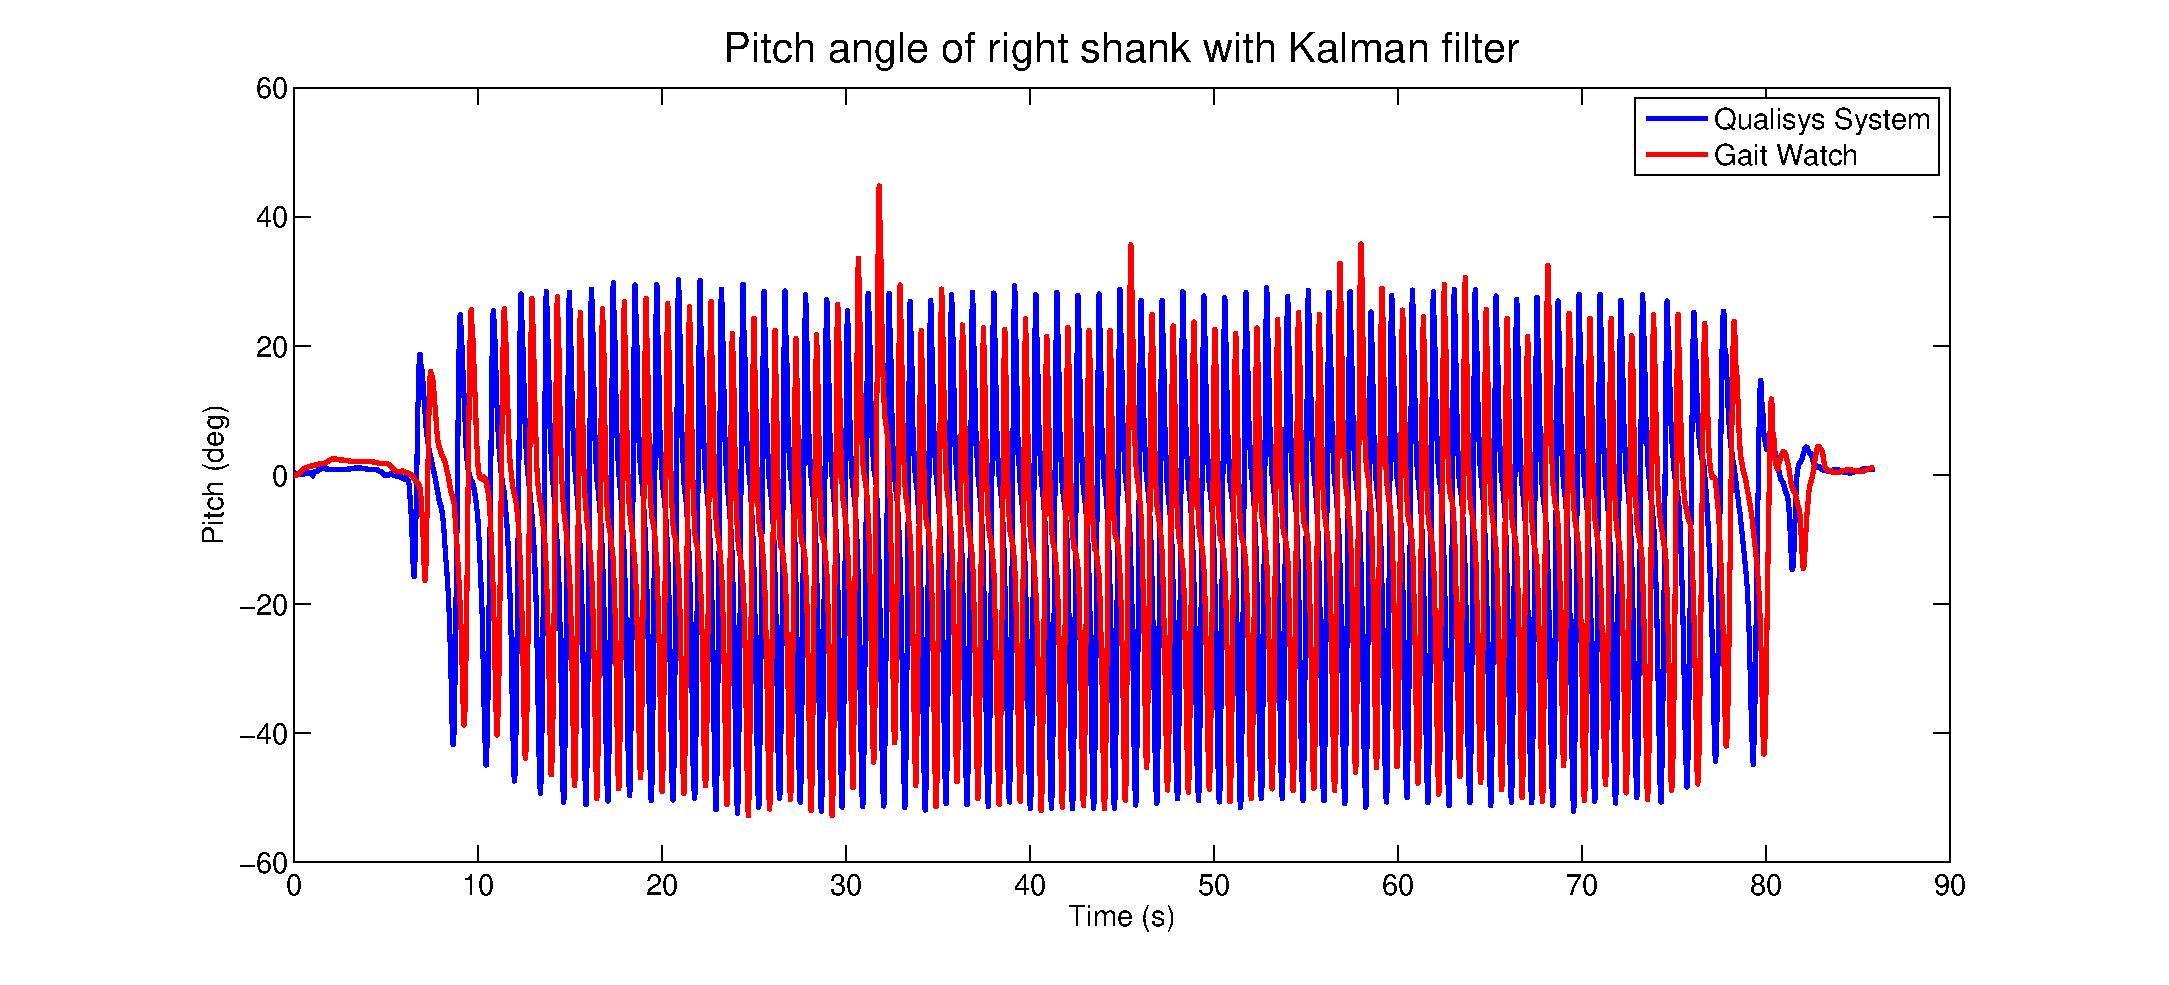
\epsfig{file=figures/QSvsGW/signalGWQS, width=1\textwidth}
	\caption{Pitch angle of right shank for 4Km/h of speed.}
	\label{fig:signalGWQS}
\end{figure}

The next step is the feature extraction. We have to differentiate two comparisons. Firstly, we are going to compare the pitch calculated with inertial sensors (GW) and infrared cameras (QS), so we will extract some specific characteristics to do this. After that, we are going to compare the angle obtained in function of the speed with which the subjects walk on the treadmill.
\begin{figure}[H]
	\centering
	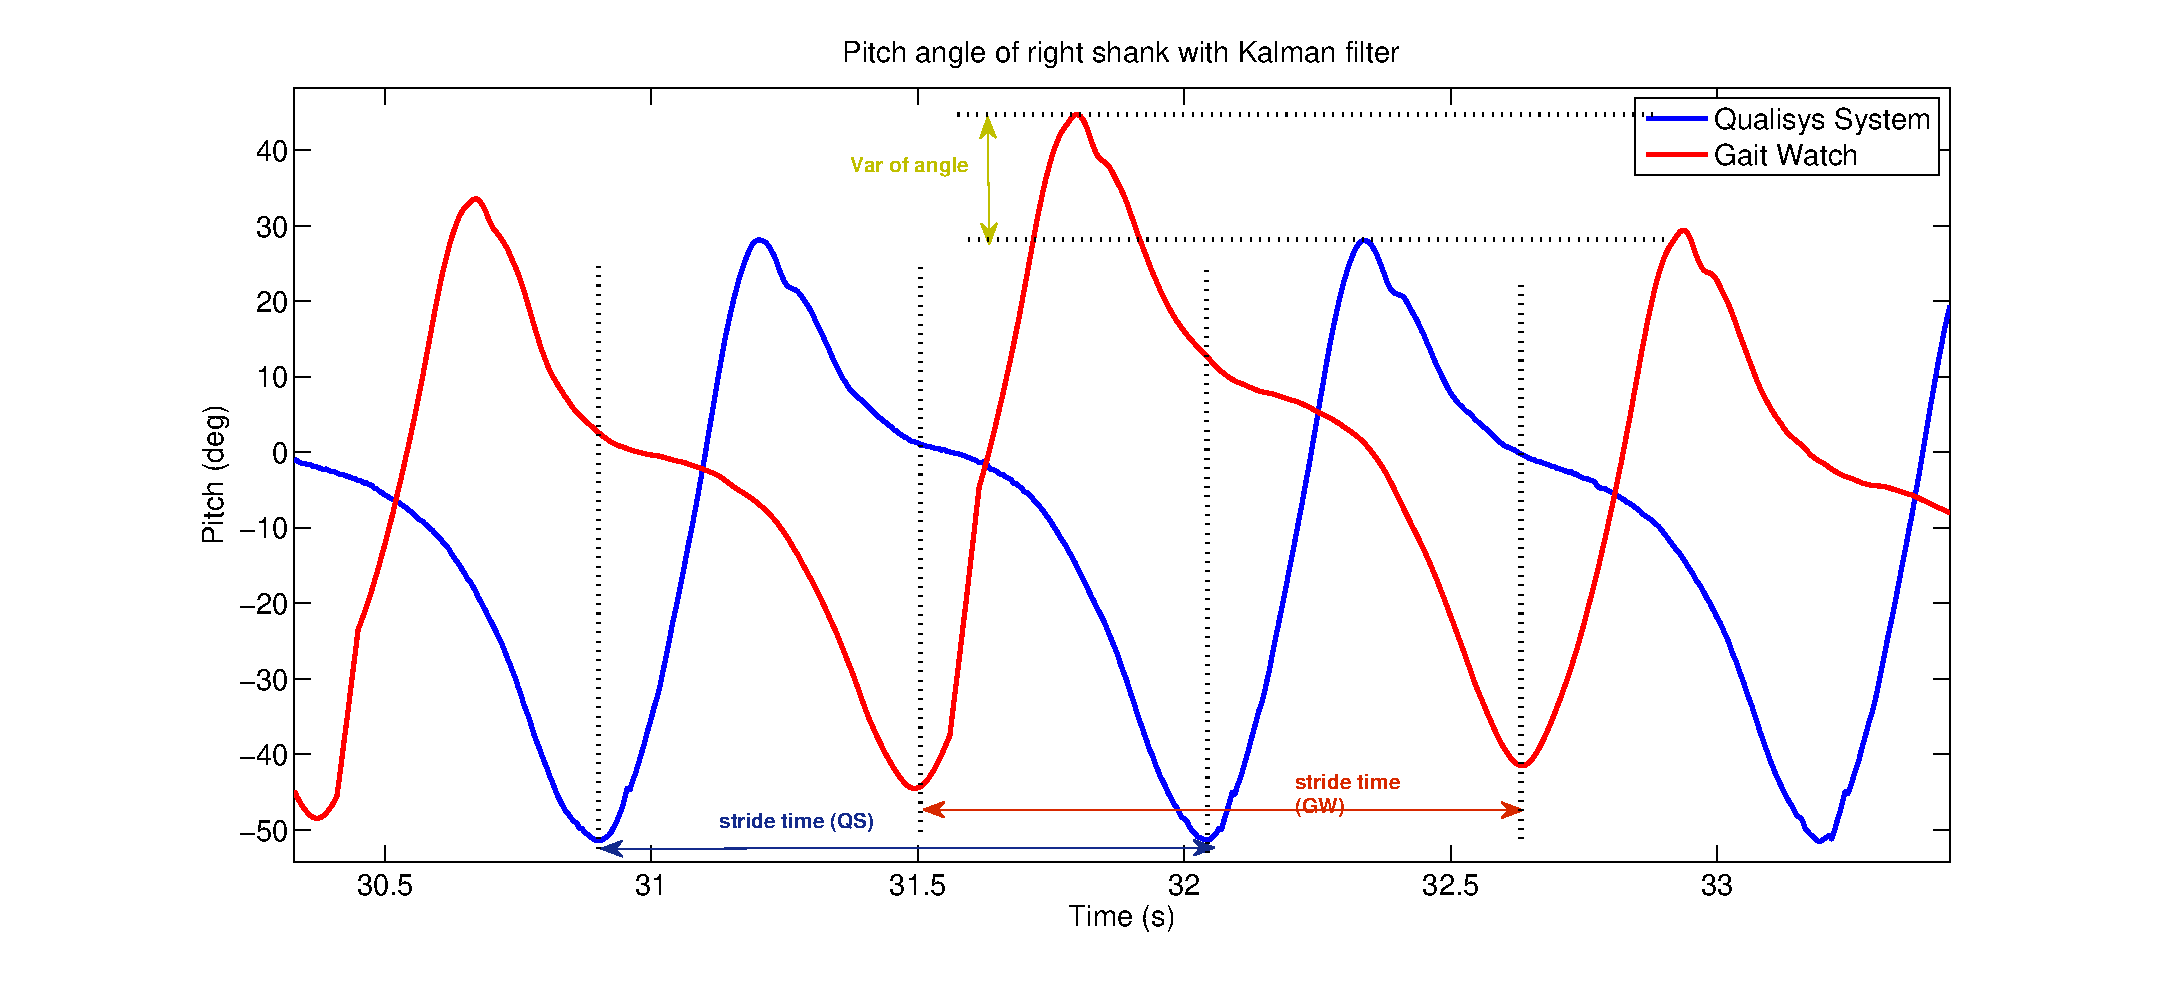
\epsfig{file=figures/QSvsGW/features_GWQS, width=1\textwidth}
	\caption{Features for pitch angle in GW and QS signals.}
	\label{fig:featuresGWQS}
\end{figure}
The first feature computed was the ‘stride time’ \ref{fig:featuresGWQS}. This is the time that a person needs to carry out a step, i.e the time since the foot is lifted from the treadmill until the moment when the same foot touches the ground and gains momentum to step again. In the pitch signal, we determine this by detecting the distance between two negative values of the pitch because the negative values happen when the segment (shank or thigh) are behind the trunk, this is just before stepping.

Other important aspect is the difference of angle obtained in both systems. We calculate values positives as well as negatives and finally obtain the mean of the difference of all them \ref{fig:featuresGWQS}.


\section{Results discussion}
Once the features have been calculated, we proceeded with the comparison between them. Firstly we can see the differences between ‘stride time’ in GW and QS signals in \ref{fig:mean_stride_time}. This figure shows the differences between them are minor so we would use the GW in place of QS with regard to this variable.

\begin{figure}[H]
	\centering
	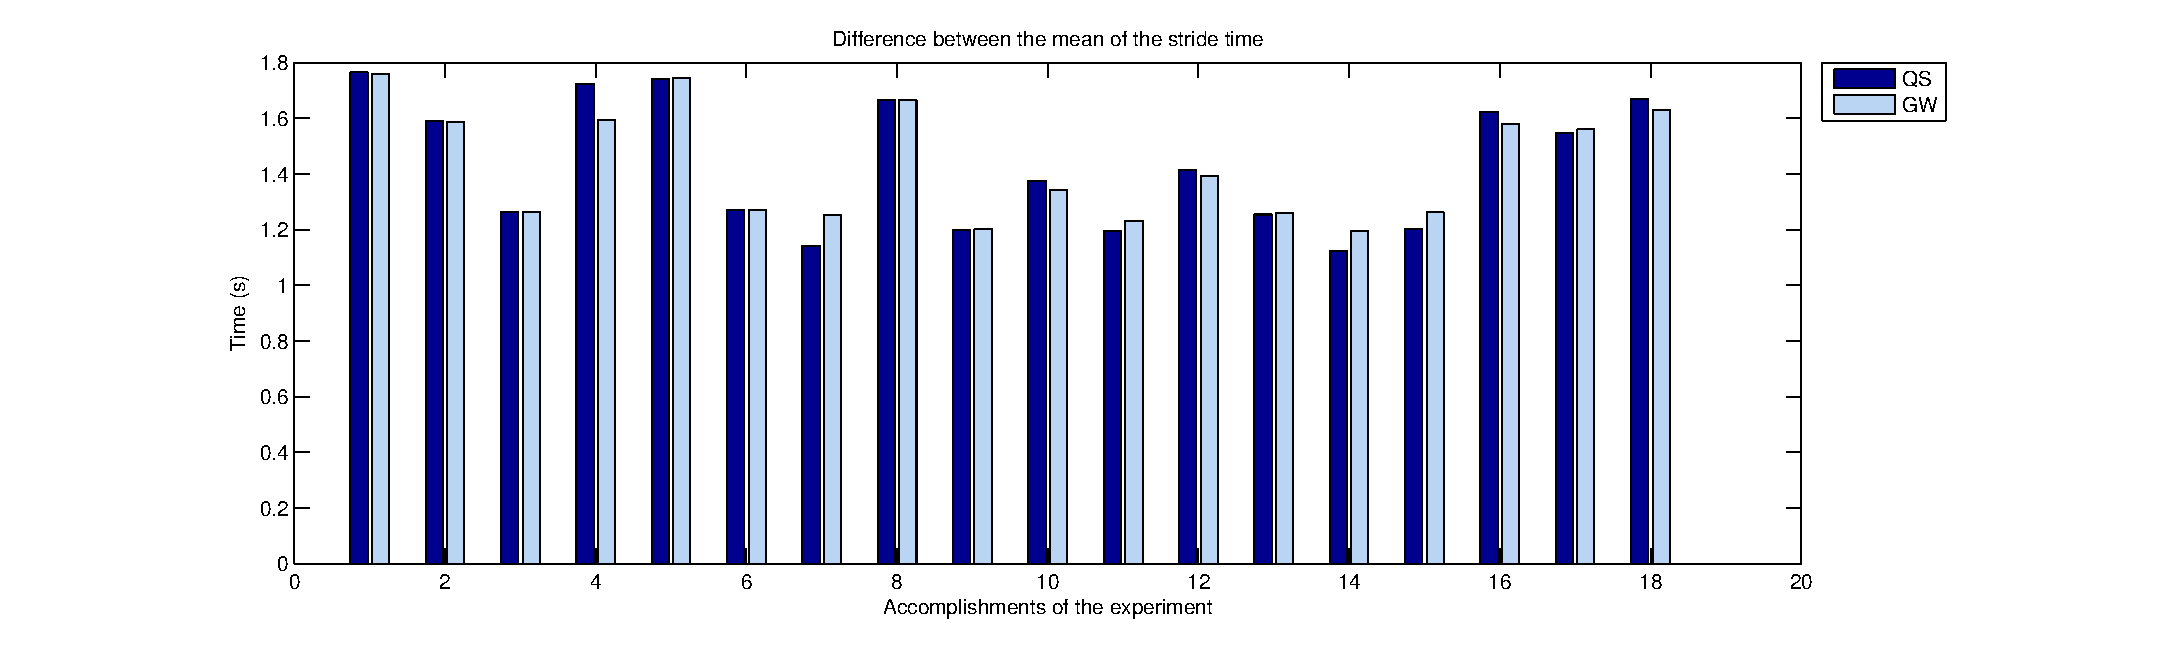
\epsfig{file=figures/QSvsGW/mean_stride_time, width=1\textwidth}
	\caption{Mean of the stride time for GW and QS signals.}
	\label{fig:mean_stride_time}
\end{figure}

‘Stride time’ is a feature used in a lot of experiments to characterise the movement because it is an interesting aspect that represents the time that a specific person needs to step. Also, it can be used for a classification between patients and control subjects, like in others studies \cite{Hausdorff}.
In our case, the difference between  the ‘stride time’ between both systems is very small. If we observe \ref{tab:Stride_time}, we can see that the greatest value of difference between systems is 0.1287 seconds.

\begin{table}[h]
	\caption{Comparison of the stride time and angle difference between GW and QS}	
	\centering
	\begin{tabular}{|c|c|c|}\hline
		
		Accomplishments & Difference Stride Time	& Difference Angle	 	\\ \hline
		1  & 0,006402343	 & 1,62502323 \\
		2 & 0,00214919	& 2,119358046 \\
		3 & 0,002432735	& 3,166649918 \\
		4 & 0,128717949	& 1,983148998 \\
		5 & 0,004818214	& 2,418373859 \\
		6 & 0,000302102	& 2,884211822 \\
		7 & 0,109688664	& 2,000748905 \\
		8 & 0,000282755	& 2,606004581 \\
		9 & 0,000604613	 & 0,644265922 \\
		10 & 0,034118318	& 2,093221696 \\
		11 & 0,038589012	& 2,597329501 \\
		12 & 0,022069119	& 0,039397798 \\
		13 & 0,004924869	& 2,771227548 \\
		14 & 0,069355008	& 2,87790541 \\
		15 & 0,059470686	& 2,227618016 \\
		16 & 0,041612352	& 0,511020994 \\
		17 & 0,012348426	& 1,834745133 \\
		18 & 0,039846301	& 1,701994772 
	\\ \hline
	\end{tabular}
	\label{tab:Stride_time}
	
\end{table}

\begin{table}[h]
	\caption{Features for different speeds}	
	\centering
	\begin{tabular}{|c|c|c|c|}\hline
		
		Speed & Stride time Diff Average & Stride time var Average & Angle Diff Average	 	\\ \hline
		2  & 1,6894	 & 0,00086 & 2,36 \\
		4 & 1,2397	& 0,017 & 4,1521\\
		6 & 1,4479 & 0,0094	& 4,6219
		\\ \hline
	\end{tabular}
	\label{tab:speeds}
	
\end{table}

In addition, it has been obtained the variations between the mean of the variance of the ‘stride time’. This parameter gives us information about the accuracy of both systems to calculate the pitch angle during the experiment.

In the majority of the accomplishments of the experiments, the variance of the GW system is greater than QS \ref{fig:var_stride_time}. It is probably due to the noise of the inertial sensors and the accuracy to calculate the pitch. However, they are very low values so it is not an important aspect that determines the quality against each other. 

\begin{figure}[H]
	\centering
	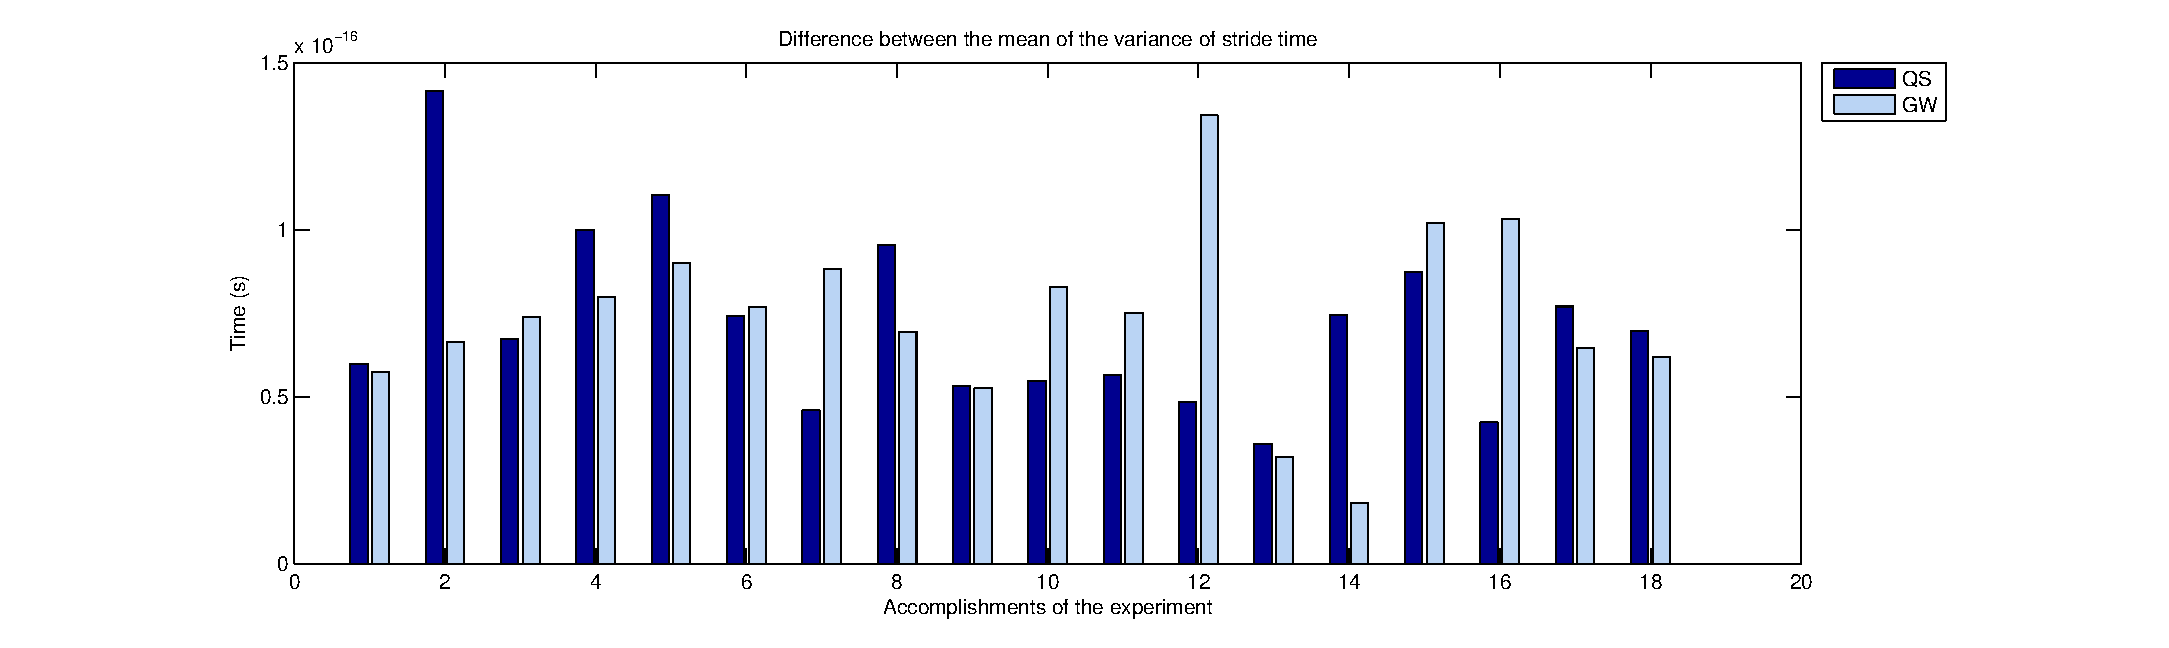
\epsfig{file=figures/QSvsGW/var_stride_time, width=1\textwidth}
	\caption{Mean of the stride time variance for GW and QS signals.}
	\label{fig:var_stride_time}
\end{figure}

Now, we will compare the mean of the angle in each experiment. The result of this is depicted in \ref{fig:mean_angle}. It is clear that the differences are not large. The greatest value of difference between angles is 3.16 degrees\ref{tab:Stride_time}. If we calculate the percentage with respect to the total average, this is about 12\% of the angle. This precision might be important depending on the application. In general, it is not a significant value to characterise the movement. Therefore, Gait Watch system may be used to substitute the Qualisys systems as a good alternative regarding the accuracy, price and portability.

\begin{figure}[H]
	\centering
	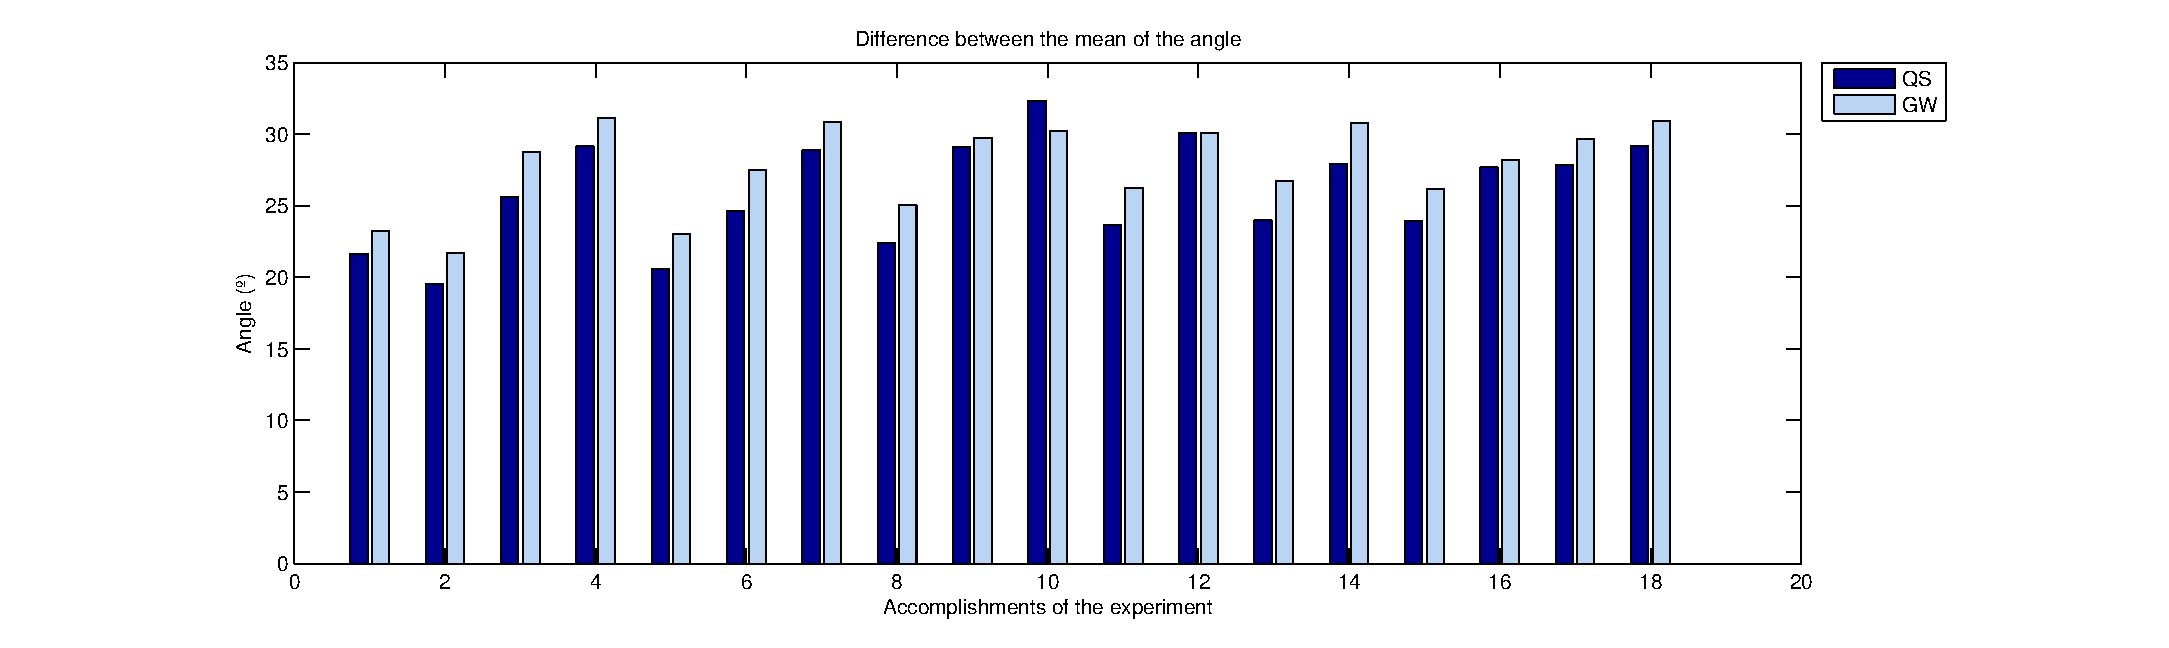
\epsfig{file=figures/QSvsGW/mean_angle, width=1\textwidth}
	\caption{Mean of the angle for GW and QS signals.}
	\label{fig:mean_angle}
\end{figure}

Then, we will see what happens when we analyse the signals with regard to different speeds. In \ref{fig:speed_stride_time}, we can see the mean of stride time for speeds of 2, 4 and 6 Km/h. If we have a look at the points represented in the picture, it seems that the ‘stride time’ is greater for low speeds than high speeds although it depends on the subject. In \ref{tab:speeds} it is shown the mean of all values for each velocity. The average ‘stride time’ is higer for 6Km/h than 4Km/h. However it does not happen in general. Therefore, we would need more measurements to establish a final conclusion.

\begin{figure}[H]
	\centering
	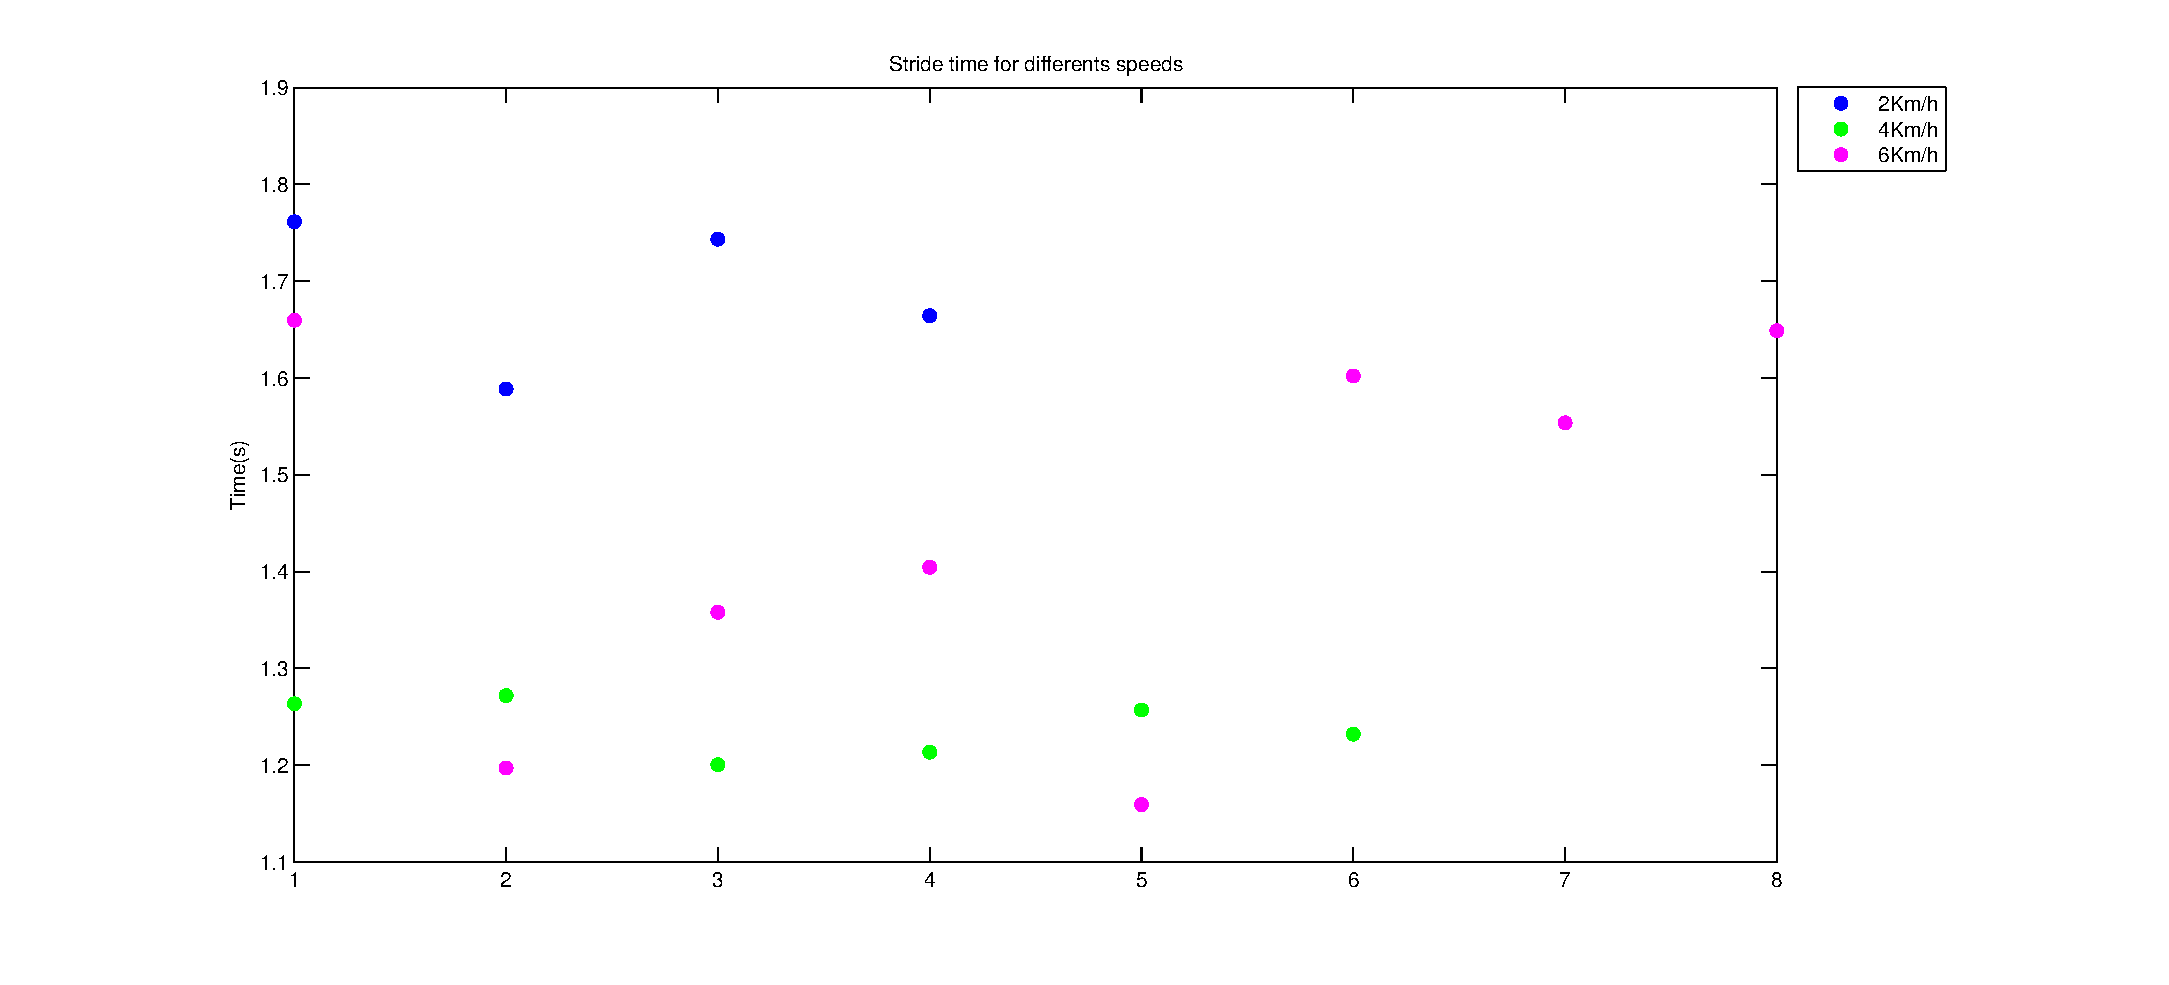
\epsfig{file=figures/QSvsGW/speed_stride_time, width=1\textwidth}
	\caption{Mean of stride time difference for each speeds.}
	\label{fig:speed_stride_time}
\end{figure}

\begin{figure}[H]
	\centering
	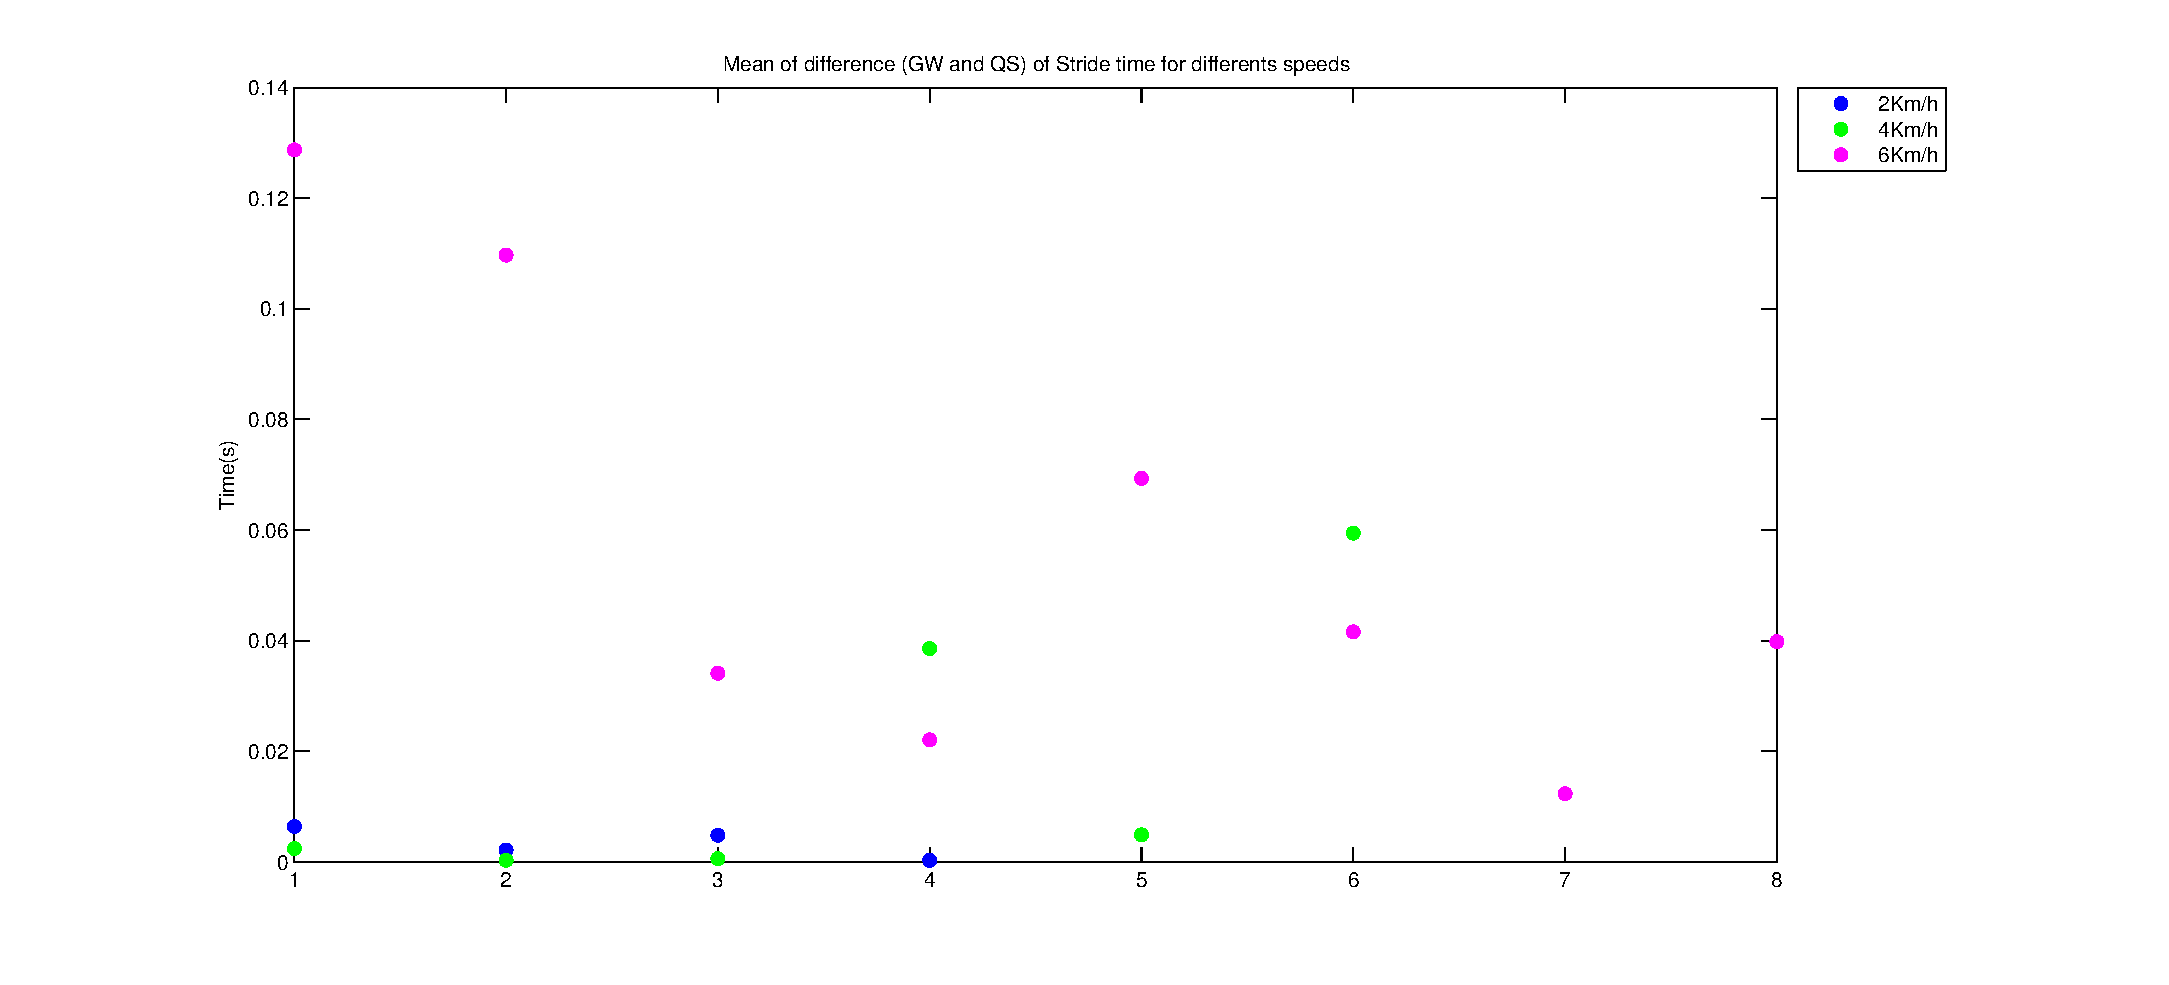
\epsfig{file=figures/QSvsGW/speed_var_stride_time, width=1\textwidth}
	\caption{Mean of stride time variance for each speeds.}
	\label{fig:speed_var_stride_time}
\end{figure}

If we scan \ref{fig:speed_var_stride_time}, we can appreciate the differences between the variance of ‘stride time’. Also, the mean of the values for each speed are put in the table \ref{tab:speeds} and the variance increases as the speed does it as well.

It is the same with the difference of the angle between systems \ref{fig:speed_angle}. The difference between angles increases with speed. So, it is an aspect that we have to consider to use the GW in place of QS.

\begin{figure}[H]
	\centering
	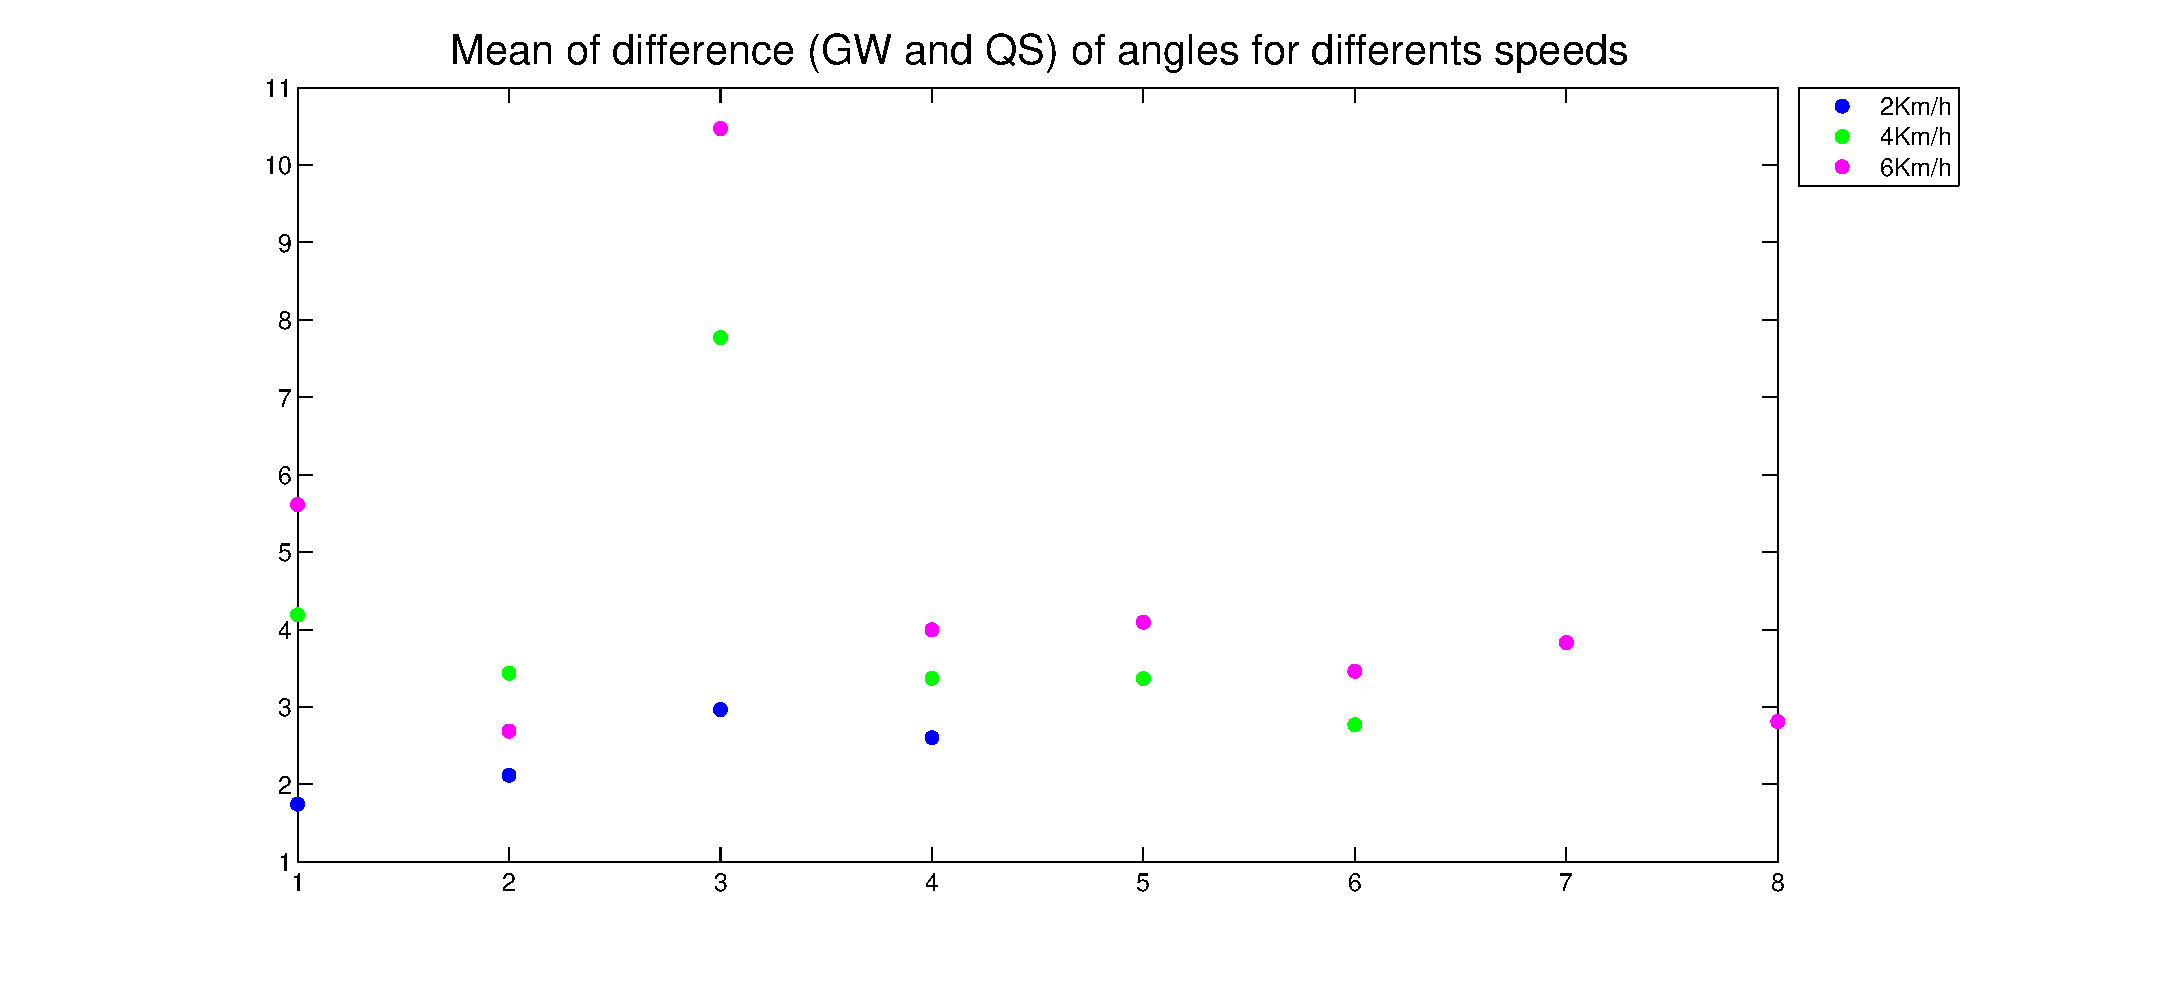
\epsfig{file=figures/QSvsGW/speed_angle, width=1\textwidth}
	\caption{Mean of angle difference for each speeds.}
	\label{fig:speed_angle}
\end{figure}


		
	\clearemptydoublepage
	\chapter{Potential Applications}
\label{ch:Applications}

After doing a study about the different systems to monitor and analyse the postural adjustments, we proceed to explain possible applications in the real life.

The force plate system is a very accurate system to analyse disorders in the patients, however it is a limited system for its price and portability. So, its applications make restricted to diagnosis some diseases.
The same happens with Qualisys System because it is necessary fixed cameras to record data. However it is a interesting way to observe data in real time with precision and robustness .

But, without a doubt, Gait Watch System is one of the most interesting system due to portability and its amount of fields where it can be used such as telerehabilitation, daily activities and performance of some athletics. This is why, the majority of applications will be focused in this system.

All of these implementations will be briefly explained below as well as a business idea as a concrete application of this Project.

\section{Diseases}
There exists a large amount of diseases that distort the motor control of human body or present symptoms that can be identified by the analysis of human body posture and motion. Along this section,  we will briefly comment how our study has influence in that.

\subsection{Telehabilitation}
\subsection{Neurological and Muscular diseases}
\subsection{Sleep disorder}

\section{Dialy activities }

\subsection{Tracking of old people}
\subsection{Athletics}

\section{Business plan }
	\clearemptydoublepage
	\chapter{Conclusions and Future Work}
\label{ch:Conclusions}
\section{Conclusion}
The analysis of posture and human body motion  has gained special relevance within the past years in many medicine fields, as well as in others kinds of applications. Traditionally, this analysis has been carried out by Force Plates and systems base on cameras of high speed using infrared markers. This fact has restricted the fields of applications due to the price, portability and limitations of visibility. For this reason, we have carried out a comparative study of these systems in contrast with low cost devices based on magnetic and inertial MEMS microsensors (Gait Watch).

To do that, we have applied different techniques and procedures that we have explained and compared along the project.
In addition, our work has a direct application, not only in diagnosis of Parkinson’s disease, but also in neurological and muscular diseases such as Multiple Sclerosis, Cerebral Palsy and Epilepsy. In the application field, we focus on the analysis of posturographic  Body-sway to detect disorders in Parkinson patients as well as falls in elderly people which are becoming increasingly frequent.

Finally, we proceed to analyze the initial objectives that were enumerated in the introductory chapter to determine to what degree they have been fulfilled.


\begin{itemize}
\item \textbf{Synchronisation}

-	One of the objectives in this section is to carry out the synchronisation between FP and GW signals. We have several signals from both systems: force, AP-COP, ML-COP, etc. in the FP system and acceleration, angular velocity, pitch, roll, etc. in the GW system, having both systems a different sample frequency. Thus, the procedure is: choose the appropriate signals to do the synchronisation, detect a common point between them and interpolate them.
After a deep analysis of these signals, we concluded that the best signal to do the synchronisation is the acceleration of the shanks and the force over the platform because you can detect in both signals when the patient touches the platform and finally do a appropriate matching.
In addition, we compare the synchronisation done with the acceleration and angular velocity of the shanks obtaining a similar result that indicates this a good procedure to do the synchronisation.

-	Other goal emerged during the development of the project is the comparison between FSD (Framed Spectrum Detector) and LTSD (Long Term Spectral Detector) algorithm to determine the intensity motion. We determined after doing the comparison that LTSD is a better method for our signals because it is designed to work under condition where the SNR is low, i.e the signal presents large noise. In our case, we want to detect the different cycles in the GW signals that correspond to each repetition so the different peaks of activity inside each period can be a problem to do the detection correctly because they are interpreted as noise by the detector. Thus, the LTSD method is more interesting for this type of signal.


\item \textbf{APA analysis}

-	One of the main goals of this project is to analyse the APAs and determine whether there is a pattern that allows us to characterise the movement before gait. The signals used for this were the acceleration and angular velocity of the trunk and the center of pressure obtained from the force measures of the force plate. The conclusion is that we can see a pattern in all these signals and also it can be detected when the patient starts to step with the right or left foot. This is a great advance because we can obtain information and extract features of these signals.

-	Analysing the state of the art we can find that there are several articles that show what and how the features are extracted. Typically, the features more used to characterise this kind of movement are the peak of acceleration and COP. We used these features  as well as other peaks in these signals that we considered that could be interesting. Also, we calculated the duration of the APA in COP, acceleration signals and gyroscope signals.

-	We focus on the PCA method to extract features because it allows us the reduction of redundant information and the interpretation of multiple gait signals. We extract the same features mentioned above before and after applying PCA. We conclude that the acceleration and angular velocity can be substituted by only one of them because there is not variance between them. This is an important conclusion when we have a big data base. 
Also, we used PCA between patients, being this the first step to do a classification in a future work.

-	If we focus in chapter\ref{ch:GWandFP}, we can determine that there is a significant correlation of some of the features calculated between FP and GW signals. Although  we should expand the data base before drawing a definitive conclusion, we could say it is possible that devices based on inertial sensors can replace platforms. This would allow to do a lot of different experiments without limitations of space and price.

\item \textbf{Classification of force data}

One of the main goals in this experiment is to determine whether it is possible to classify Parkinson patients and healthy subjects from force data. We tested two different methods to extract features: PCA (unsupervised) and PLS (supervised) using SVM as classifier. The conclusion of this is: firstly, PCA is more appropriate from an accuracy viewpoint and PLS has better results than PCA from a sensitivity viewpoint, secondly we can obtain a good classification with both methods. This allows us to conclude that the analysis could be used to help in the diagnostic of Parkinson's disease.

\item \textbf{Qualisys system and Gait Watch (treadmill experiment)}

-	An initial objective was to determine what kinds of features we could extract in this type of experiment. The signals used to analyse this behaviour are the pitch angle of shanks and thighs. Thus, we concluded that the most interesting aspects to consider were ‘stride time’, variance of ‘stride time’  and peaks of angles. ‘Stride time’ has been a feature used with success in other similar studies so we though that it could be a significant parameter.

-	Determining the accuracy of the pitch angle obtained with GW and QS systems was another of our targets. To do this, we compare the features calculated from the pitch. The conclusion is that we can use the GW in place of QS in the majority of the cases if we need accuracy in the angle and ‘stride time’ because the difference of both is minimal.

-	In addition, we compare both systems in different conditions of speed to determine if the velocity affects in the accuracy of the systems. After the study, we can say that speed influences in the variance of ‘stride time’ and angle, i.e when the speed is higher the difference between systems to calculate the ‘stride time’ and angle increases. 
\end{itemize}

\section{Future Work}
As we have done for the final conclusions, we proceed to analyze future work for the two main parts of our system.

\begin{itemize}
\item \textbf{Force Plate and Gait Watch (experiment with Parkinson patients over a platform)}

- We will increase the data base of the patient for achieving results more accurately. Currently, we have a limited data base with only five patients. This gives us a rough guidance of the information that we can obtain but it is not decisive because to reach a definitive conclusion we have to have at least twenty patients.

-	We will add control subjects to our data base. The fact of having patients of Parkinson’s disease as well as control subjects would allow to do a classification. This is very important because it would really help in medical diagnosis of this disease.
The classification can be achieved through a SVM which separates a given labeled training dataset with a hyperplane that is maximally distant from the two classes, being these classes the patients and control subjects (or patients with different levels of the disease). The objective is to build a function using training data that will correctly classify new examples.

- We will test others kinds of algorithms to obtain features of the gait data. One of them is ICA (Independent Component Analysis).  ICA is a statistical technique that represents multidimensional random vector as a linear combination of nongaussian random variables (independent component) that are as independent as possible. ICA is somewhat similar to PCA to extract features. However, it would be interesting to compare both ICA and PCA to determine if we can extract the same information using both methods. 

- In addition, all the work developed in this project could be used in other applications. For example in patients with motor disorders or elderly people and establish if this study can be a widespread procedure to others fields.

\item \textbf{Classification of force data}

The classification has been done with force data while subjects (both patients and control subjects) were walking normally. We will try to do the classification with other types of experiments where subjects are carrying out different activities. It would allow us to extend the study to whatever daily activity.

\item \textbf{Qualisys system and Gait Watch (treadmill experiment)}

-	As in the first case, we will increase the data base. This not only allows to have more accurate results but also we can do others types of studies to deepen the knowledge of the Posturographic Body-sway  with inertial data.

-	We will analyse the movements not only of shanks and thighs but also of trunk and arms carrying out other experiments with Qualisys System and Gait Watch.
	
\end{itemize}
	
	\clearemptydoublepage
	\bibliographystyle{unsrt}
	\bibliography{biblio}
	\clearemptydoublepage
	\begin{titlepage}
	\label{ch:Appendices}
	
{ \huge \bfseries Appendices \\[1.0 cm] }

\end{titlepage} 
	
	\clearemptydoublepage
\end{document}